\section{Objetivos}

\subsection{Objetivo General}
Explicar y comprender experimentalmente cómo se puede determinar la relación carga-masa del electrón, la técnica de difracción para medir el grosor de un cabello, y el funcionamiento del interferómetro de Michelson-Morley, detallando cada proceso y su importancia en la física moderna.

\subsection{Objetivos Específicos}
\begin{itemize}
    \item Explicar la metodología para calcular la relación carga-masa del electrón usando un tubo de vacío esférico que contiene un cañón de electrones y placas deflectoras. Para ello, se detalla cómo un campo magnético uniforme creado por bobinas de Helmholtz influye en la trayectoria de los electrones y permite calcular dicha relación.
    \item Describir el uso de patrones de difracción para medir el grosor de un cabello humano, explicando cómo un haz de luz láser produce estos patrones al atravesar el cabello.
    \item Analizar el principio de interferencia y la sensibilidad del interferómetro de Michelson-Morley, explicando cómo los patrones de interferencia se afectan al cambiar la distancia en las trayectorias ópticas. Esto permite ilustrar el concepto de interferencia de ondas y la aplicación del interferómetro en experimentos de precisión.
\end{itemize}

\section{Marco Teórico}
La física moderna aborda conceptos fundamentales que explican los fenómenos a nivel microscópico y macroscópico, revelando la naturaleza ondulatoria y partícula de la materia y la energía. Los experimentos en este laboratorio son cruciales para entender teorías fundamentales como la cuántica y la relatividad especial.

\subsection{Relación Carga-Masa del Electrón}
El experimento de la relación carga-masa del electrón demuestra cómo los campos magnéticos afectan las trayectorias de partículas cargadas. Un campo magnético perpendicular a la velocidad de un electrón lo desvía en una trayectoria circular, según la fuerza de Lorentz:
\[
F = qvB = \frac{mv^2}{r}
\]
donde \(q\) es la carga del electrón, \(v\) su velocidad, \(B\) el campo magnético, y \(r\) el radio de la trayectoria circular.

\subsection{Emisión de Luz por Gases Ionizados}
La excitación de átomos de gases bajo un campo eléctrico y su posterior emisión de luz es un fenómeno que se estudia tanto en física atómica como en astrofísica, proporcionando una ventana a la composición y características de objetos astronómicos distantes.

\subsection{Difracción para Medir el Grosor de un Cabello}
La difracción ocurre cuando una onda de luz encuentra un obstáculo de dimensiones comparables a su longitud de onda. La fórmula para determinar el grosor del cabello a través de la difracción es:
\[
d = \frac{\lambda L}{\Delta y}
\]
donde \(\lambda\) es la longitud de onda del láser, \(L\) la distancia de la pantalla, y \(\Delta y\) el espaciamiento entre los máximos de interferencia.

\subsection{Interferómetro de Michelson-Morley}
Este dispositivo fue fundamental para refutar la existencia del éter y es esencial para experimentos que requieren alta precisión en la medición de distancias. El interferómetro divide un haz de luz en dos, enviando cada uno en direcciones perpendiculares y luego reuniéndolos para crear un patrón de interferencia que depende de las diferencias en el recorrido óptico:
\[
\Delta x = \frac{\lambda}{2\pi} \Delta \phi
\]
donde \(\Delta \phi\) es la diferencia de fase entre los dos haces.


\section{Experimentos}
\subsection{Experimento 1: Relación Carga-Masa del Electrón}
Este experimento demuestra cómo los campos magnéticos afectan las trayectorias de partículas cargadas, como los electrones. Utilizando un campo magnético perpendicular a la velocidad de un electrón, se observa que el electrón se desvía en una trayectoria circular, un fenómeno descrito por la fuerza de Lorentz.

\subsubsection{Datos Experimentales}
Utilizando diferentes potenciales aceleradores, medimos los radios de las órbitas que los electrones describen bajo la influencia del campo magnético. Los datos son los siguientes:

\begin{center}
\begin{tabular}{|c|c|c|c|c|c|}
\hline
\textbf{Radio de la órbita / Potencial Acelerador} & \textbf{100V} & \textbf{150V} & \textbf{200V} & \textbf{250V} & \textbf{300V} \\
\hline
r1 = 0.02 m & 7.13 & 20.4 & 24.1 & 26.8 & 30.2 \\
r2 = 0.03 m & 2.24 & 13.03 & 15.92 & 17.87 & 19.7 \\
r3 = 0.04 m & 0.34 & 9.5 & 11.52 & 13.9 & 14.77 \\
r4= 0.05 m & 0 & 7.57 & 9.2 & 10.36 & 11.66 \\
\hline
\end{tabular}
\end{center}

\subsubsection{Análisis de la Pendiente}
La pendiente de las curvas en la gráfica de $\text{Potencial Acelerador}$ vs $\text{Radio de la órbita}$ representa la relación carga-masa del electrón, $\left(\frac{e}{m}\right)$. Este parámetro es crucial ya que describe cómo la fuerza magnética afecta a un electrón en función del potencial acelerador aplicado. Las pendientes calculadas de las cuatro series de datos son:

\begin{figure}[H]
  \centering
  \begin{subfigure}[b]{\textwidth}
      \centering
      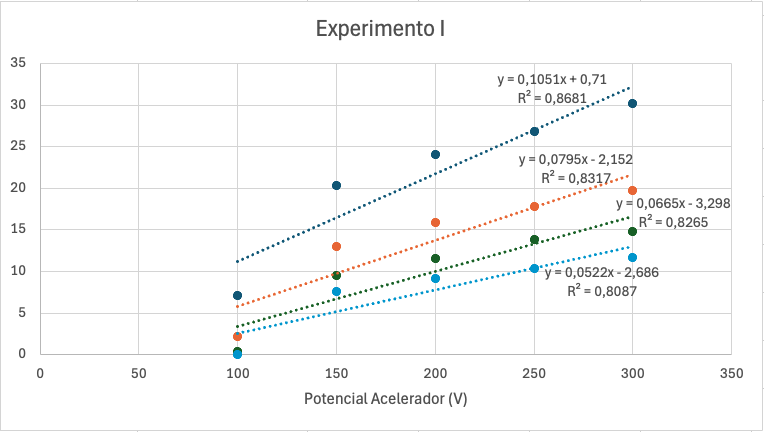
\includegraphics[width=0.9\textwidth]{Figures/1. Content/grafica-experimento-1.png}
      \caption{Gráfica del experimento 1}
      \label{fig: Grafica del experimento 1}
  \end{subfigure}
  \hfill
\end{figure}

\begin{itemize}
    \item Para r1 = 0.02 m: pendiente = 0.1015
    \item Para r2 = 0.03 m: pendiente = 0.0795
    \item Para r3 = 0.04 m: pendiente = 0.0655
    \item Para r4 = 0.05 m: pendiente = 0.0522
\end{itemize}

Cada pendiente refleja cómo el radio de la trayectoria varía con el aumento del potencial, y es inversamente proporcional al cuadrado de la masa del electrón multiplicado por su carga.

\subsubsection{Implicaciones en la Física Moderna}
El experimento no solo proporciona una manera de calcular la relación carga-masa del electrón, sino que también ejemplifica conceptos fundamentales de la física moderna, como el electromagnetismo y la mecánica cuántica. La habilidad de medir con precisión cómo los campos magnéticos afectan a partículas cargadas tiene implicaciones importantes en áreas como la espectroscopia, la computación cuántica y la investigación de plasmas.

\subsection{Experimento 2: Emisión de Luz por Gases Ionizados}

En este experimento, se observó la emisión de luz como resultado de la excitación de gases ionizados, utilizando diferentes gases y analizando las líneas espectrales emitidas. Estas líneas son características de cada elemento y permiten identificar la composición del gas.

\subsubsection{Datos Experimentales y Análisis}
Utilizando un espectrómetro, medimos las posiciones de las líneas espectrales emitidas por diferentes elementos y las comparamos con los valores teóricos conocidos. Esto permite confirmar la identidad de cada gas basado en sus firmas espectrales.

\begin{figure}[H]
  \centering
  \begin{subfigure}[b]{\textwidth}
      \centering
      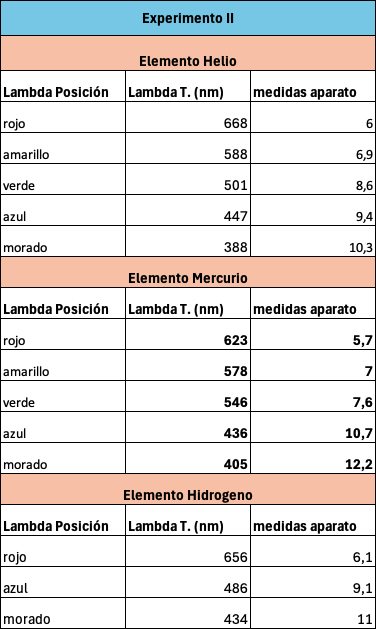
\includegraphics[width=0.43\textwidth]{Figures/1. Content/tabla-experimento-2.png}
      \caption{Tabla de valores del experimento 2}
      \label{fig: Tabla experimento 2}
  \end{subfigure}
  \hfill
\end{figure}

\begin{itemize}
    \item \textbf{Helio (He)}
    \begin{itemize}
        \item Rojo: \( \lambda = 668 \, \text{nm} \)
        \item Amarillo: \( \lambda = 588 \, \text{nm} \)
        \item Verde: \( \lambda = 501 \, \text{nm} \)
        \item Azul: \( \lambda = 447 \, \text{nm} \)
        \item Morado: \( \lambda = 388 \, \text{nm} \)
    \end{itemize}
    \item \textbf{Mercurio (Hg)}
    \begin{itemize}
        \item Rojo: \( \lambda = 623 \, \text{nm} \)
        \item Amarillo: \( \lambda = 578 \, \text{nm} \)
        \item Verde: \( \lambda = 546 \, \text{nm} \)
        \item Azul: \( \lambda = 436 \, \text{nm} \)
        \item Morado: \( \lambda = 405 \, \text{nm} \)
    \end{itemize}
    \item \textbf{Hidrógeno (H)}
    \begin{itemize}
        \item Rojo: \( \lambda = 656 \, \text{nm} \)
        \item Azul: \( \lambda = 486 \, \text{nm} \)
        \item Morado: \( \lambda = 434 \, \text{nm} \)
    \end{itemize}
\end{itemize}


\[
\text{Porcentaje de Error para cada Elemento:}
\]
\[
\text{Helio: } \left|\frac{632.816 - 668}{632.816}\right| \times 100\% \approx 5.56\%
\]
\[
\text{Mercurio: } \left|\frac{691 - 623}{691}\right| \times 100\% \approx 9.84\%
\]
\[
\text{Hidrógeno: } \left|\frac{656.3 - 656}{656.3}\right| \times 100\% \approx 0.05\%
\]

\subsubsection{Análisis de Gráficas}
Las gráficas de dispersión muestran la relación entre la posición medida en el espectrómetro y la longitud de onda teórica para cada línea espectral. La pendiente de la línea de tendencia indica la calibración del espectrómetro, sugiriendo que las medidas son consistentes a través del espectro visible.

\begin{figure}[H]
  \centering
  \begin{subfigure}[b]{\textwidth}
      \centering
      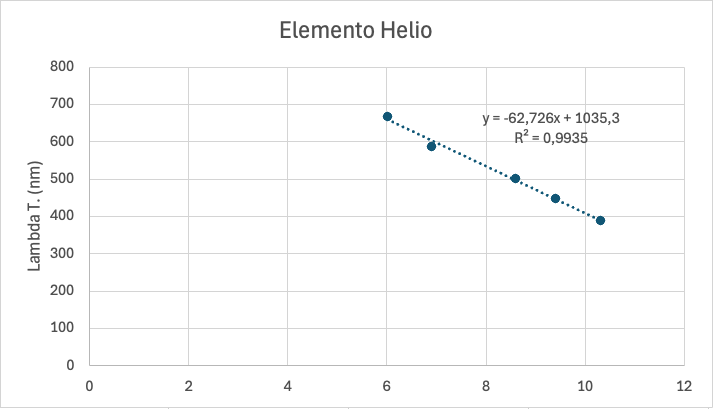
\includegraphics[width=0.7\textwidth]{Figures/1. Content/grafica-experimento-2-helio.png}
      \caption{Gráfica del Helio}
      \label{fig: Grafica del Helio}
  \end{subfigure}
  \hfill
\end{figure}

\begin{figure}[H]
  \centering
  \begin{subfigure}[b]{\textwidth}
      \centering
      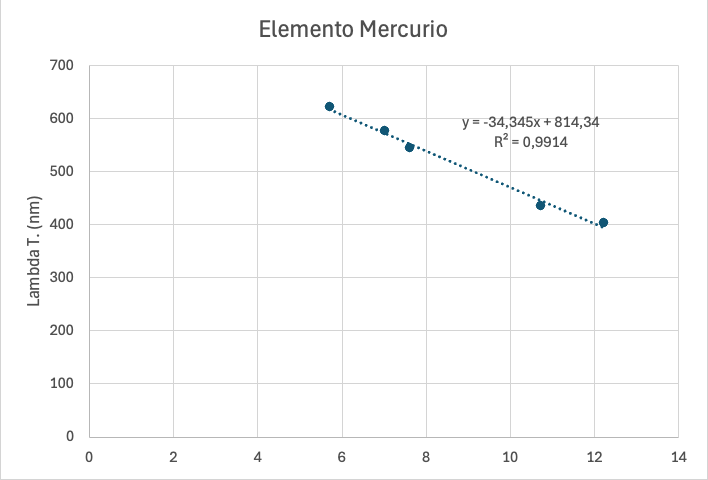
\includegraphics[width=0.6\textwidth]{Figures/1. Content/grafica-experimento-2-mercurio.png}
      \caption{Gráfica del Mercurio}
      \label{fig: Grafica del Mercurio}
    \end{subfigure}
  \hfill
\end{figure}

\begin{figure}[H]
  \centering
  \begin{subfigure}[b]{\textwidth}
      \centering
      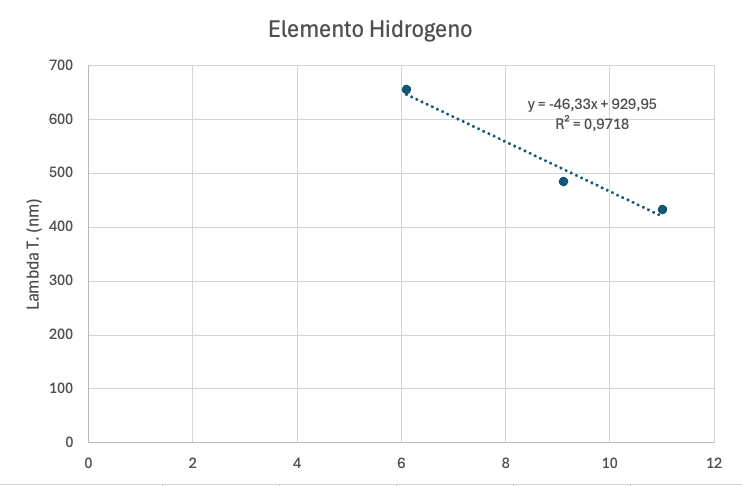
\includegraphics[width=0.7\textwidth]{Figures/1. Content/grafica-experimento-2-hidrogeno.png}
      \caption{Gráfica del Hidrógeno}
      \label{fig: Grafica del Hidrogeno}
  \end{subfigure}
  \hfill
\end{figure}

\subsubsection{Conclusión sobre Identificación de Elementos}
Identificamos los elementos como Helio, Mercurio, e Hidrógeno al comparar las longitudes de onda medidas con los valores teóricos conocidos, confirmando la identidad de los gases.

\subsubsection{Relación con la Física Moderna}
Este experimento demuestra la importancia de la espectroscopia, una herramienta crucial en física moderna y astrofísica, para identificar la composición química de materiales y cuerpos celestes.

\subsection{Experimento 3: Medición del Grosor de un Cabello}
En este experimento, aplicamos el principio de difracción de la luz para medir el grosor de un cabello humano. La luz láser, al pasar a través de un cabello, produce un patrón de difracción, y a partir de este patrón podemos calcular el diámetro del cabello utilizando la relación entre la longitud de onda del láser, la distancia entre las franjas claras de difracción y la distancia desde el cabello hasta la superficie donde se proyecta el patrón.

\begin{figure}[H]
  \centering
  \begin{subfigure}[b]{\textwidth}
      \centering
      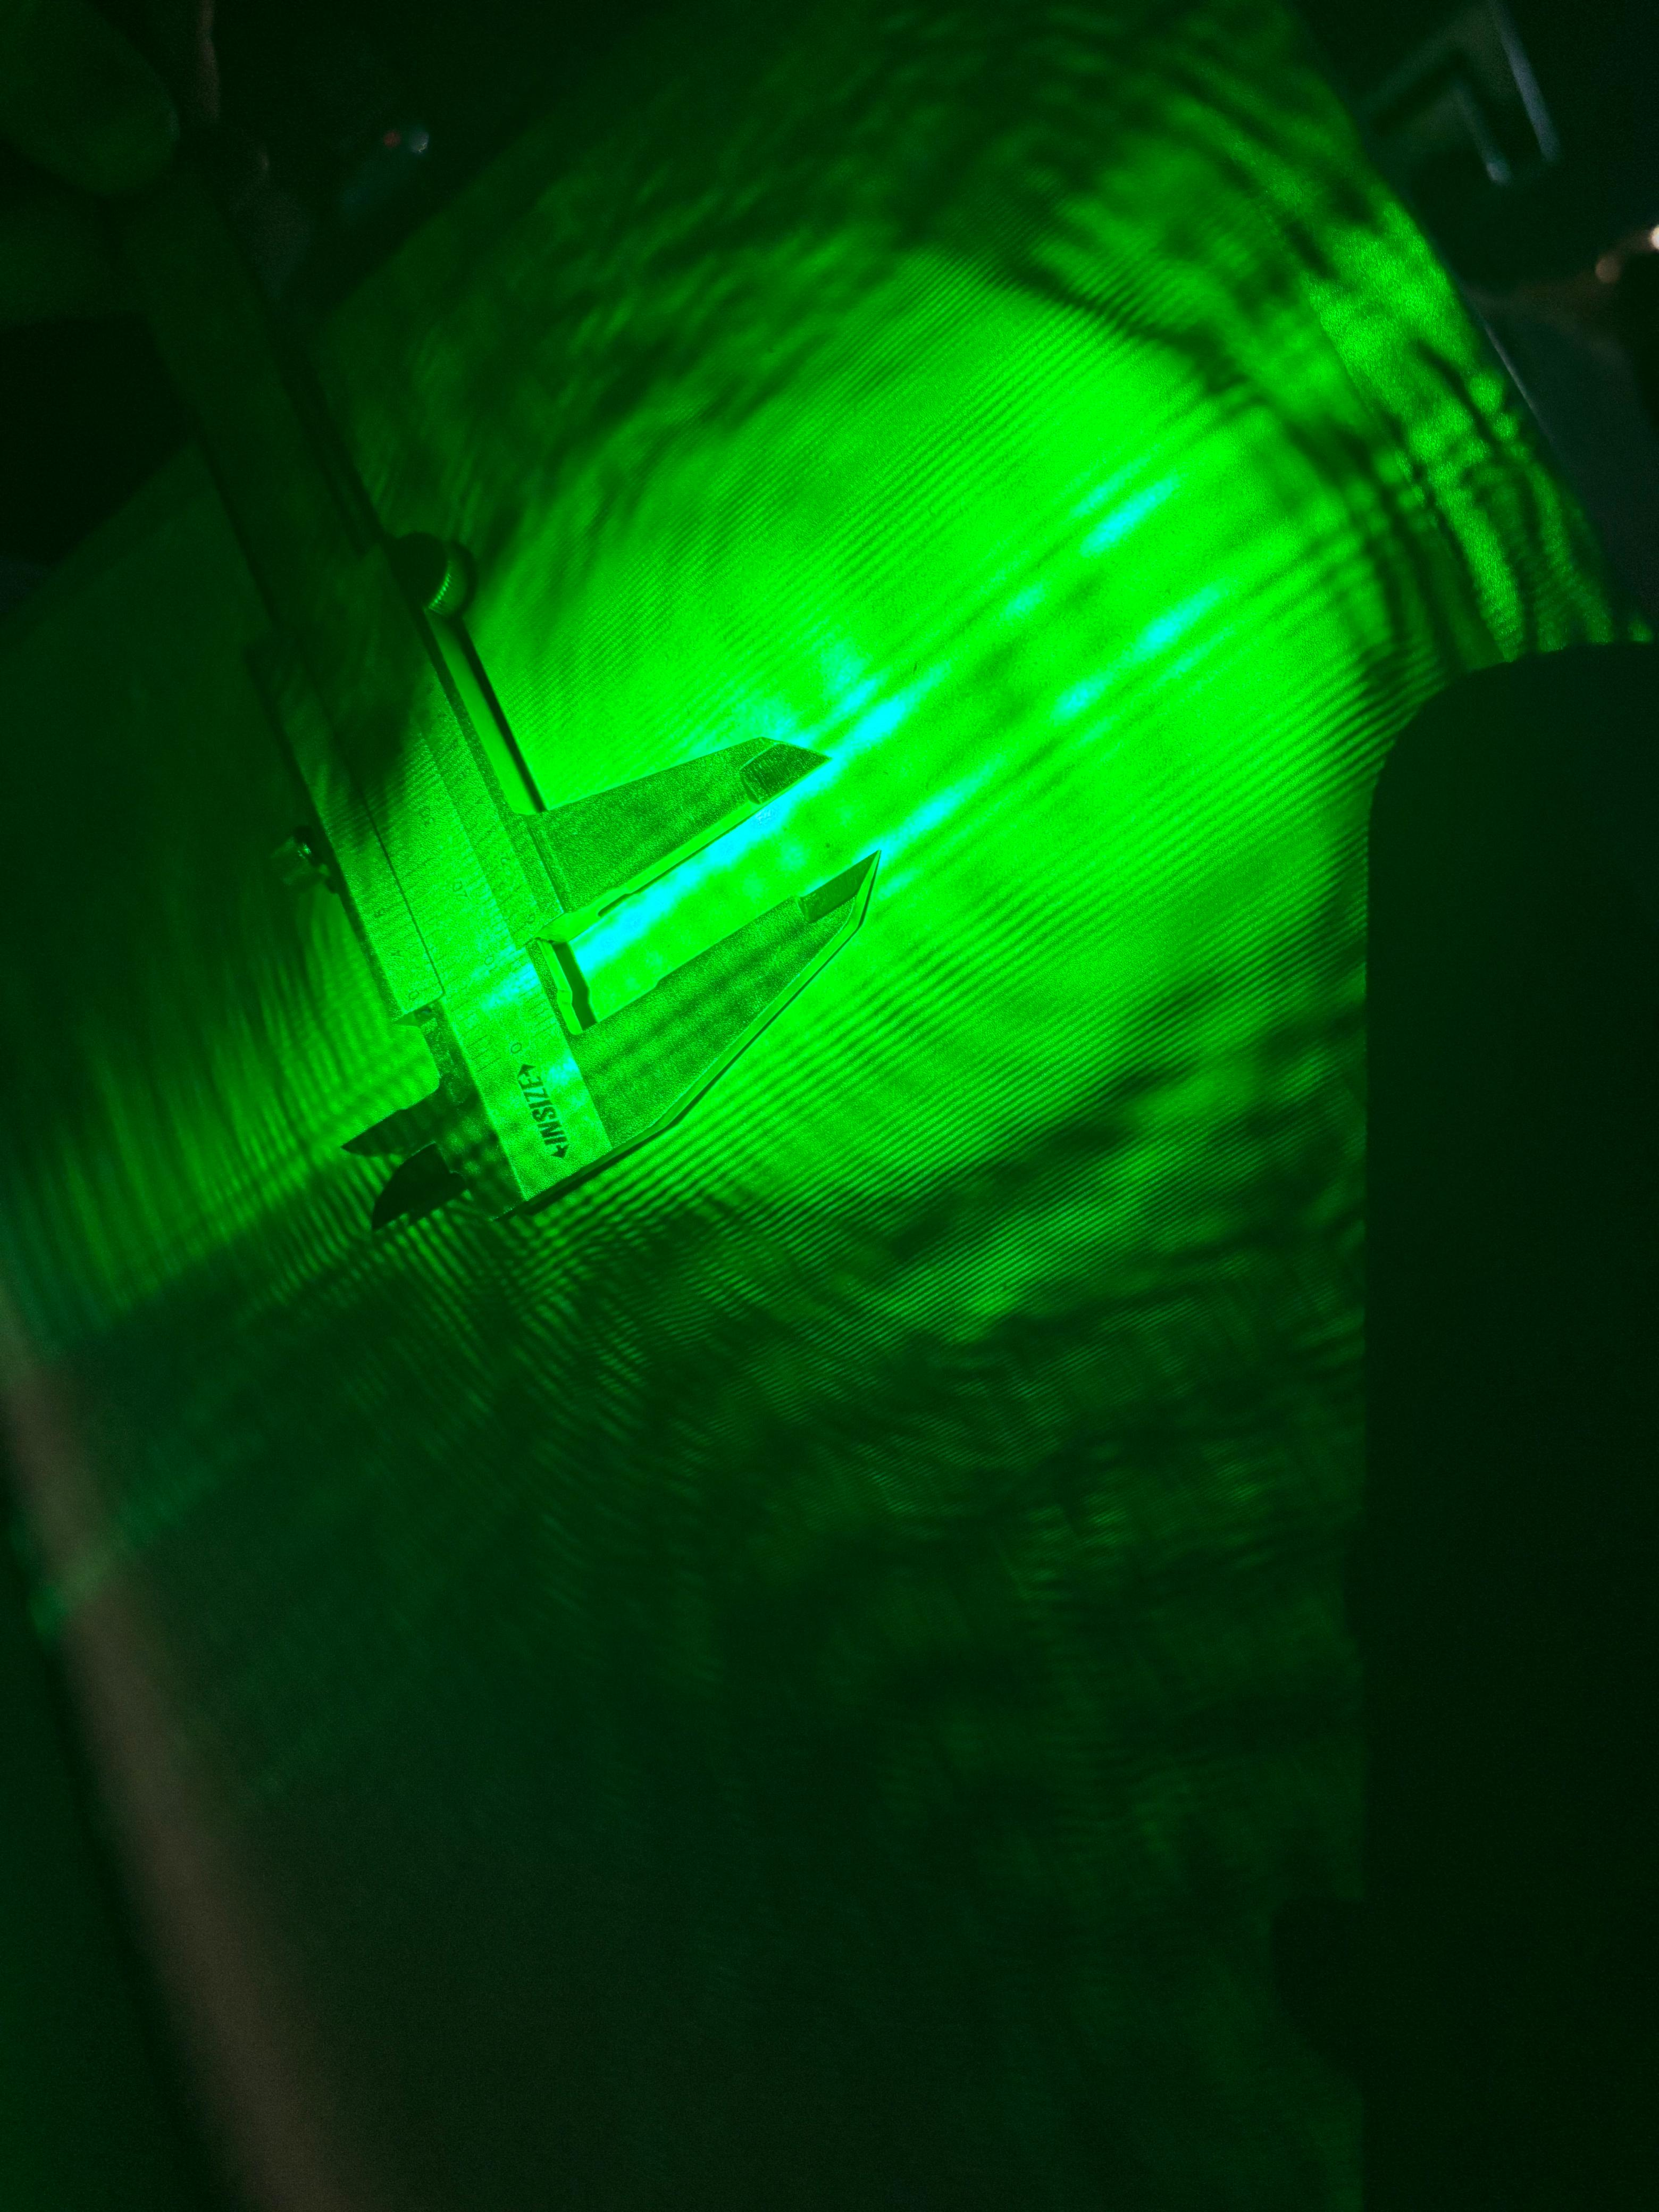
\includegraphics[width=0.4\textwidth]{Figures/1. Content/experimento-3.jpeg}
      \caption{Evidencias de medición}
      \label{fig: Evidencias de medicion 3}
  \end{subfigure}
  \hfill
\end{figure}

\subsubsection{Datos Experimentales}

\begin{figure}[H]
  \centering
  \begin{subfigure}[b]{\textwidth}
      \centering
      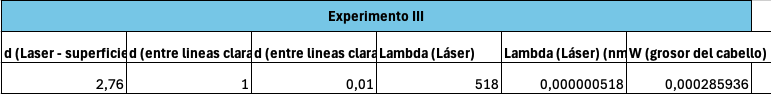
\includegraphics[width=\textwidth]{Figures/1. Content/tabla-experimento-3.png}
      \caption{Tabla de valores del experimento 3}
      \label{fig: Tabla experimento 3}
  \end{subfigure}
  \hfill
\end{figure}

\begin{itemize}
    \item Distancia del láser a la superficie \(d\): \(2.76 \, \text{m}\)
    \item Distancia entre las líneas claras observadas en el patrón de difracción \(d\): \(0.01 \, \text{m}\)
    \item Longitud de onda del láser \(\lambda\): \(518 \, \text{nm} = 0.000000518 \, \text{m}\)
\end{itemize}

\subsubsection{Cálculo del Grosor del Cabello}
Utilizando la fórmula para la difracción de la luz por un cabello:
\[
d = \frac{\lambda L}{\Delta y}
\]
donde:
\begin{itemize}
    \item \(L\) es la distancia desde el cabello hasta la superficie de proyección.
    \item \(\Delta y\) es la distancia entre las franjas de difracción.
    \item \(\lambda\) es la longitud de onda del láser.
\end{itemize}
Sustituyendo los valores obtenemos:
\[
W = \frac{0.000000518 \times 2.76}{0.01} \approx 0.000143 \, \text{m} = 143 \, \text{micrómetros}
\]

\subsubsection{Análisis de Error}
Considerando el rango típico para el grosor del cabello humano, calculamos los porcentajes de error:
\begin{itemize}
    \item Grosor máximo estimado: \(170 \, \text{micrómetros}\)
    \[
    \text{Error} = \left| \frac{143 - 170}{170} \right| \times 100\% \approx 15.88\%
    \]
    \item Grosor promedio del cuero cabelludo: \(110 \, \text{micrómetros}\)
    \[
    \text{Error} = \left| \frac{143 - 110}{110} \right| \times 100\% \approx 30\%
    \]
    \item Grosor típico en individuos asiáticos: \(120 \, \text{micrómetros}\)
    \[
    \text{Error} = \left| \frac{143 - 120}{120} \right| \times 100\% \approx 19.17\%
    \]
\end{itemize}

\subsubsection{Relación con la Física Moderna}
Este experimento demuestra la aplicación de la teoría de la difracción de ondas, un concepto fundamental en la física moderna que se extiende al estudio de la naturaleza ondulatoria de las partículas (dualidad onda-partícula) en la mecánica cuántica. Además, la capacidad de medir dimensiones a escalas microscópicas usando principios ópticos es esencial en tecnologías de nanofabricación y caracterización de materiales en física y ingeniería. Este análisis proporciona una base para entender cómo técnicas simples pueden aplicarse para estudiar y verificar fenómenos complejos y principios en física moderna, conectando la teoría con aplicaciones prácticas y experimentales.

\subsection{Experimento 4: Interferencia de Luz con el Láser}

Este experimento involucra la medición de la longitud de onda de la luz láser mediante interferencia. Utilizando un láser de longitud de onda conocida, se crea un patrón de interferencia que nos permite calcular la longitud de onda experimental a través de la difracción de la luz en una rendija.

\begin{figure}[H]
  \centering
  \begin{subfigure}[b]{\textwidth}
      \centering
      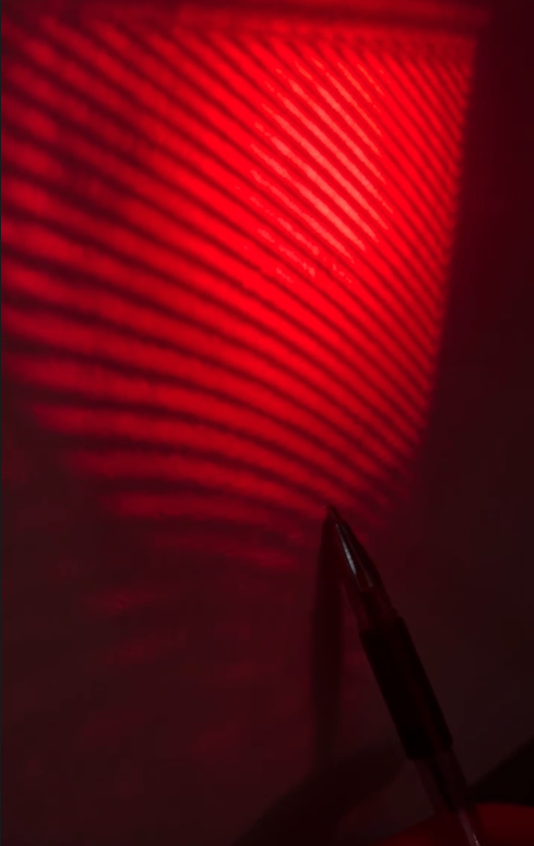
\includegraphics[width=0.4\textwidth]{Figures/1. Content/experimento-4.png}
      \caption{Evidencias de medición}
      \label{fig: Evidencias de medicion 4}
  \end{subfigure}
  \hfill
\end{figure}

\subsubsection{Datos Experimentales}

\begin{figure}[H]
  \centering
  \begin{subfigure}[b]{\textwidth}
      \centering
      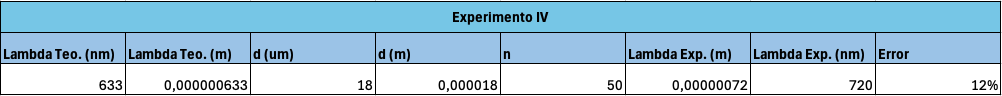
\includegraphics[width=\textwidth]{Figures/1. Content/tabla-experimento-4.png}
      \caption{Tabla de valores del experimento 4}
      \label{fig: Tabla experimento 4}
  \end{subfigure}
  \hfill
\end{figure}

\begin{itemize}
    \item Longitud de onda teórica del láser \(\lambda_{teo}\): \(633 \, \text{nm} = 0.000000633 \, \text{m}\)
    \item Distancia entre rendijas \(d\): \(18 \, \mu\text{m} = 0.000018 \, \text{m}\)
    \item Número de franjas observadas \(n\): \(50\)
    \item Longitud de onda experimental \(\lambda_{exp}\): \(720 \, \text{nm} = 0.00000072 \, \text{m}\)
\end{itemize}

\subsubsection{Cálculo del Error}
El porcentaje de error se calcula comparando la longitud de onda experimental con la teórica:
\[
\text{Error \%} = \left(\frac{\left| \lambda_{exp} - \lambda_{teo} \right|}{\lambda_{teo}}\right) \times 100\%
\]
\[
\text{Error \%} = \left(\frac{\left| 0.00000072 - 0.000000633 \right|}{0.000000633}\right) \times 100\% \approx 12\%
\]
Este error indica la precisión del montaje experimental y la alineación de la rendija y el detector.

\subsubsection{Relación con la Física Moderna}
La interferencia y difracción son fenómenos que subrayan la naturaleza ondulatoria de la luz, uno de los principios clave de la física moderna. Este experimento ilustra directamente cómo la luz, al igual que cualquier partícula cuántica, exhibe propiedades tanto de partícula como de onda (dualidad onda-partícula). El análisis de estos patrones no solo es fundamental para entender la teoría cuántica, sino también para aplicaciones como la espectroscopía y el desarrollo de tecnologías ópticas avanzadas.

Este enfoque experimental proporciona una comprensión profunda de cómo las ondas de luz interfieren entre sí y cómo esta interferencia puede ser utilizada para medir características físicas con alta precisión, lo que es crucial en campos como la metrología y las tecnologías de información cuántica.

\section{Conclusiones}
A lo largo de este laboratorio, hemos realizado varios experimentos que no solo demuestran principios fundamentales de la física moderna, sino que también destacan su aplicabilidad en contextos prácticos y tecnológicos. Cada experimento ha contribuido de manera significativa a nuestra comprensión de conceptos físicos esenciales y a nuestra capacidad para aplicar estos conceptos en la resolución de problemas complejos.

\subsection{Contribuciones y Aplicaciones}
\begin{itemize}
    \item \textbf{Relación Carga-Masa del Electrón:} Este experimento resaltó la influencia de los campos magnéticos en las partículas cargadas, una piedra angular en el estudio del electromagnetismo y la mecánica cuántica. La habilidad para determinar la relación carga-masa del electrón es crucial para el desarrollo de tecnologías que dependen de la manipulación precisa de partículas cargadas, como los aceleradores de partículas y la espectrometría de masas.
    
    \item \textbf{Difracción para Medir el Grosor de un Cabello:} Al aplicar principios de difracción, este experimento no solo confirmó la naturaleza ondulatoria de la luz, sino que también ilustró cómo la física puede utilizarse para medir dimensiones microscópicas con gran precisión. Esta técnica tiene aplicaciones directas en los campos de la nanotecnología y la biología, donde la medición precisa a escalas pequeñas es fundamental.
    
    \item \textbf{Emisión de Luz por Gases Ionizados:} La espectroscopia, explorada a través de este experimento, es esencial para la astrofísica y la física atómica, permitiendo a los científicos determinar la composición de estrellas y otros cuerpos celestes lejanos. Además, este experimento subraya cómo los modelos cuánticos de los átomos explican las líneas espectrales características, fundamentales para la química analítica y la física.
    
    \item \textbf{Interferómetro de Michelson-Morley:} La capacidad de medir minúsculas diferencias en las trayectorias de luz subraya la importancia de la interferometría en la ciencia moderna, incluyendo la relatividad especial, las pruebas de gravedad, y las tecnologías de medición de distancias como el GPS y los sistemas de posicionamiento láser.
\end{itemize}

\subsection{Conclusión General}
Los experimentos realizados demuestran la relevancia continua de la física clásica y moderna en la resolución de problemas contemporáneos y en el avance de la tecnología. Al integrar conceptos teóricos con aplicaciones prácticas, estos experimentos no solo mejoran nuestra comprensión de la física, sino que también preparan el terreno para futuras innovaciones en ciencia y tecnología. Así, este laboratorio no solo cumple con los objetivos educativos de un curso de física, sino que también inspira un mayor interés y apreciación por la ciencia fundamental y su impacto en el mundo real.
